\documentclass[12pt, letterpaper]{article}
\author{Копылов Иван Александрович}
\usepackage[T1,T2A]{fontenc}
\usepackage[utf8]{inputenc}
\usepackage[english, russian]{babel}
\usepackage{graphicx}
\usepackage{booktabs}
\usepackage{listings}
\usepackage{a4, marginfit}
\graphicspath{{images/}}

\lstset{
    basicstyle=\fontencoding{T1}\ttfamily\small,
    breaklines=true,
    columns=fullflexible,
    keepspaces=true,
    frame=single
}

\title{Численные методы одномерной оптимизации}
\date{Москва 2026}
\begin{document}
\maketitle
Лабораторная работа №1
Вариант 10

Копылов Иван Александрович, БИВТ-24-9\\

\includegraphics[width=2cm]{signature.jpg}

НИТУ МИСИС

Лычёв Андрей Владимирович
\newpage
\section{Цель работы}
Приобретение практических навыков для решения задач одномерной минимизации численными методами.
\section{Задача}
Требуется найти безусловный минимум функции одной переменной 
\begin{math}
y = f(x)
\end{math}
на отрезке 
\begin{math}
[a, b]
\end{math}, где функция является унимодальной. То есть найти такую точку
\begin{math}
x^{*} \in [a, b]
\end{math}
такую, что
\begin{math}
f(x^*) = \min\limits_{x \in [a, b]} f(x)
\end{math}
.

Согласно варианту 10,\\
\begin{math}
f(x) = \frac{-x}{e^x} \\ 
a = 0 \\ 
b = 2 \\ 
\epsilon = 0.0001
\end{math}
\begin{itemize}
    \item \textit{Метод 1} — Метод поразрядного поиска
    \item \textit{Метод 2} — Метод деления отрезка пополам
    \item \textit{Метод 3} — Метод парабол
\end{itemize}

\begin{enumerate}
    \item Составить программы поиска минимума функции тремя различными мето
дами в соответствии с заданием (язык программирования выбрать самостоя
тельно, все лабораторные работы должны быть выполнены на одном языке, 
при реализации методов запрещается пользоваться библиотечными функциями, 
которые реализуют перечисленные выше методы оптимизации).
    \item Найти координаты и значение функции в точке минимума заданными методами.
    \item Найти точное значение координаты точки минимума аналитическими методами, то есть используя необходимые и достаточные условия экстремума.
    \item Исследовать сходимость методов и провести сравнение по числу вычислений
функции для достижения заданной точности. Результаты оформить в видетаблицы.
\end{enumerate}



\section{GenAI}
\textbf{Использованные инструменты GenAI:}
\begin{enumerate}
    \item OpenAI — GPT 5.5. Использовался для прояснения деталей работы алгоритмов.
\end{enumerate}

\section{Графическое представление функции на заданном интервале}
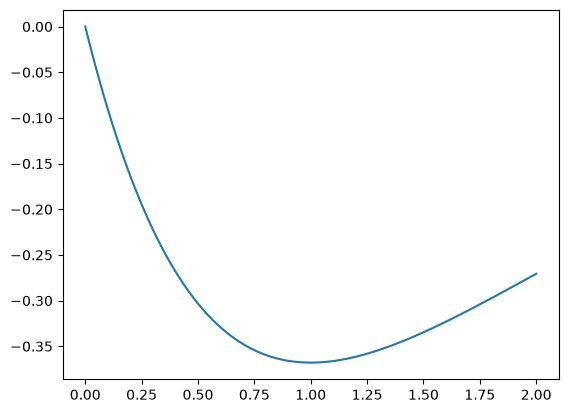
\includegraphics{func.png}

\section{Минимум функции}
Найдем минимум функции аналитическим способом
\begin{math}
    f'(x) = (\frac{-x}{e^x})' = e^(-x) * (x-1)\\
    e^(-x) * (x-1) = 0 \rightarrow
    x = 1
\end{math}

Проверим, что $x = 1$ удовлетворяет необходимому условию минимума\\
\begin{math}
    f''(x) = e^(-x) * (x-1)' = -e^(-x) (x - 2) \\
    f''(1) = -e^(-1)(-2) = 2e^(-1) > 0
\end{math}\\
$x = 1$ удовлетворяет условию минимума


Найдем значение $f(1)$:
\begin{math}
    f(1) = \frac{-1}{e^1} \approx -0,3678794412
\end{math}

\section{Листинги программ}
\begin{lstlisting}[language=Python]

import math
import matplotlib.pyplot as plt
import numpy as np

def f_base(x):
    ans = -x / math.pow(math.e, x)
    return ans

# graph
xs = np.linspace(0, 2, 100)
ys = np.array(list(map(f_base, xs)))

plt.plot(xs, ys)
plt.show()

# Incremental search method
def method_1(a, b, eps):
    iter_c = 0
    f_call_c = 0


    h = (b - a) / 4

    def f(x):
        nonlocal f_call_c
        f_call_c += 1
        return f_base(x)

    x0 = a
    f_x0 = f(x0)

    while abs(h) > eps:
        iter_c += 1

        x1 = x0 + h
        f_x1 = f(x1)

        if f_x0 > f_x1:
            x0 = x1
            f_x0 = f_x1
            if(a < x0 < b):
                continue            

        x0 = x1
        f_x0 = f_x1
        h = -h/4
    
    return (x0, f_x0, iter_c, f_call_c)

# Method of dividing the segment in half
def method_2(a, b, eps):
    iter_c = 0
    f_call_c = 0

    def f(x):
        nonlocal f_call_c
        f_call_c += 1
        return f_base(x)

    xm = (a+b)/2
    f_xm = f(xm)
    l = b - a
    
    while l > eps:
        iter_c += 1
        x1 = a + l/4
        x2 = b - l/4

        f_x1 = f(x1)
        if f_x1 < f_xm:
            b = xm
            xm = x1

        else:
            f_x2 = f(x2)
            if f_x2 < f_xm:
                a = xm
                xm = x2
            else: 
                a = x1
                b = x2

        l = b - a
    return (xm, f_xm, iter_c, f_call_c)

# Parabolic method
def method_3(a, b, eps):
    iter_c = 0
    f_call_c = 0

    def f(x):
        nonlocal f_call_c
        f_call_c += 1
        return f_base(x)
    
    f_a = f(a)
    f_b = f(b)
    c = a + (3 - math.sqrt(5)) / 2 * (b - a)
    f_c = f(c)


    while max(c - a, b - c) > 2 * eps:
        iter_c += 1
        p = math.pow(b - c, 2) * (f_a - f_c) - math.pow(c - a, 2) * (f_b - f_c)
        q = 2 * ((b - c)*(f_a - f_c) + (c - a)*(f_b - f_c))

        if q != 0 and (c + p/q) != c:
            t = c + p/q
        else:
            t = (a + c) / 2
        f_t = f(t)

        
        if t < c:
            if f_t < f_c:
                b = c
                f_b = f_c
                c = t
                f_c = f_t
            else: 
                a = t
                f_a = f_t
        else:
            if f_t < f_c:
                a = c
                f_a = f_c
                c = t
                f_c = f_t
            else: 
                b = t
                f_b = f_t

    return (c, f_c, iter_c, f_call_c)

a = 0
b = 2
eps = 0.0001

(xm_1, f_xm_1, iter_c_1, f_call_c_1) = method_1(a, b, eps)
print(iter_c_1, f_call_c_1, xm_1, f_xm_1)

(xm_2, f_xm_2, iter_c_2, f_call_c_2) = method_2(a, b, eps)
print(iter_c_2, f_call_c_2, xm_2, f_xm_2)

(xm_3, f_xm_3, iter_c_3, f_call_c_3) = method_3(a, b, eps)
print(iter_c_3, f_call_c_3, xm_3, f_xm_3)
\end{lstlisting}

\section{Результаты вычислений}
\begin{center}
    \small
   \resizebox{\textwidth}{!}{%
   \begin{tabular}{l c c c c}
        \hline
        Название & Число & Количество вычислений & Найденное & Значение \\
        метода & итераций & функции & решение & функции \\
        \hline
        Минимум & ~ & ~ & 1.0 & -0,3678794412 \\
        Метод 1 (ПП) & 33 & 34 & 1.0001220703 & -0.3678794384 \\
        Метод 2 (ДОП) & 15 & 31 & 1.0 & -0.3678794412 \\
        Метод 3 (парабол) & 16 & 19 & 1.0000000121 & -0.3678794412 \\
    \end{tabular}% 
   }
\end{center}
\section{Сраунительная характеристика методов}
Все три метода оказались неожиданно близки по производительности.

Хуже всех показал себя метод поразрядного поиска с точностью Х только до 4 знака после запятой и наибольшими и числом итераций, и кол-вом вычислений функции.

Из-за особенностей исследуемой функции метод деления отрезка пополам сразу дал идеально точный ответ (1.00).
Одновременно это привело к тому, что каждую итерацию этот метод был вынужден проводить сразу два выисления функции, что существенно повысило его вычислительную сложность.
Если бы 2 вычисления были бы необходимы только в половине итераций, метод ДОП приблизился бы по скорости к методу парабол.

Метод парабол показал достаточно хороший результат с точностью до 5 знака после запятой по Х и наименьшим кол-вом вычислений функции.

\section{Выводы} 
Исходя из результатов данного эксперимента можно предположить, что метод ДОП и метод парабол примерно эквивалентны по вычислительной сложности и получаемой точности.

\section{Проверка предположения}
Проведём идентичное исследование для той же функции на интервале от 0 до 3.
\begin{center}
    \small
   \resizebox{\textwidth}{!}{%
   \begin{tabular}{l c c c c}
        \hline
        Название & Число & Количество вычислений & Найденное & Значение \\
        метода & итераций & функции & решение & функции \\
        \hline
        Минимум & ~ & ~ & 1.0 & -0,3678794412 \\
        Метод 1 (ПП) & 32 & 33 & 1.0001220703  & -0.3678794384 \\
        Метод 2 (ДОП) & 15 & 23 & 0.9999847412 & -0.3678794411 \\
        Метод 3 (парабол) & 39 & 42 & 1.0000000166 & -0.3678794411 \\
    \end{tabular} %
   }
\end{center}
Забавно. И метод ДОП, и метод парабол имеют крайне высокую степень точности, но при этом метод парабол требует почти в два раза больше вычислений.
\end{document}